% ****** Start of file apssamp.tex ******
%
%   This file is part of the APS files in the REVTeX 4.1 distribution.
%   Version 4.1r of REVTeX, August 2010
%
%   Copyright (c) 2009, 2010 The American Physical Society.
%
%   See the REVTeX 4 README file for restrictions and more information.
%
% TeX'ing this file requires that you have AMS-LaTeX 2.0 installed
% as well as the rest of the prerequisites for REVTeX 4.1
%
% See the REVTeX 4 README file
% It also requires running BibTeX. The commands are as follows:
%
%  1)  latex apssamp.tex
%  2)  bibtex apssamp
%  3)  latex apssamp.tex
%  4)  latex apssamp.tex
%
\documentclass[%
 reprint,
%superscriptaddress,
%groupedaddress,
%unsortedaddress,
%runinaddress,
%frontmatterverbose, 
%preprint,
%showpacs,preprintnumbers,
%nofootinbib,
%nobibnotes,
%bibnotes,
 amsmath,amssymb,
 aps,
%pra,
%prb,
%rmp,
%prstab,
%prstper,
%floatfix,
]{revtex4-1}

\usepackage{graphicx}% Include figure files
\usepackage{dcolumn}% Align table columns on decimal point
\usepackage{bm}% bold math
\usepackage{tabulary}
%\usepackage{hyperref}% add hypertext capabilities
%\usepackage[mathlines]{lineno}% Enable numbering of text and display math
%\linenumbers\relax % Commence numbering lines

%\usepackage[showframe,%Uncomment any one of the following lines to test 
%%scale=0.7, marginratio={1:1, 2:3}, ignoreall,% default settings
%%text={7in,10in},centering,
%%margin=1.5in,
%%total={6.5in,8.75in}, top=1.2in, left=0.9in, includefoot,
%%height=10in,a5paper,hmargin={3cm,0.8in},
%]{geometry}

\def \sc {\em Saccharomyces cerevisiae}
\renewcommand\tablename{TABLA}
\begin{document}

%\preprint{APS/123-QED}

\title{An\'alisis cr\'itico de dos modelos de explicaci\'on para la regla de centralidad-letalidad en redes proteicas de  \sc}% Force line breaks with \\
\thanks{A footnote to the article title}%

\author{Emanuel Chironi}
% \altaffiliation[Also at ]{Physics Department, XYZ University.}%Lines break automatically or can be forced with \\
\author{Federico}%
\author{Lucas Alonso}
% \altaffiliation[Also at ]{Physics Department, XYZ University.}%Lines break automatically or can be forced with \\
\author{Francisco}
% \altaffiliation[Also at ]{Physics Department, XYZ University.}%Lines break automatically or can be forced with \\ 
\email{Second.Author@institution.edu}
\affiliation{%
Universidad de Buenos Aires\\
Redes complejas\\
Trabajo Computacional N° 2\\
}%


%\collaboration{CLEO Collaboration}%\noaffiliation

%\date{\today}% It is always \today, today,
             %  but any date may be explicitly specified

\begin{abstract}
La regla de centralidad y letalidad es un ejemplo de relaci\'on entre funcionalidad biol\'ogica y topolog\'ia de redes, la cual ha sido reportada por la literatura especializada. Sin embargo, el origen de tal comportamiento permanece elusivo. Al respecto, se han propuesto distintas hip\'otesis para intentar explicar la regla. En este trabajo se revisan cr\'iticamente dos de esos modelos, a partir de la reconstrucci\'on de los pasos dados por Zotenko y sus colaboradores, en la revisi\'on de ambas hip\'otesis. Para eso se utilizaron cuatro redes de interacci\'on de prote\'inas de la levadura {\sc}. Se testearon ambas hip\'otesis a partir de los datos extra\'idos de las cuatro redes mencionadas y se obtuvieron resultados parcialmente an\'alogos a los reportados por Zotenko y colaboradores. En consecuencia, se concluy\'o que la primera  hip\'otesis analizadas deber\'ia descartarse, pero que la evidencia no era suficiente para descartar la segunda.
\end{abstract}

%\pacs{Valid PACS appear here}% PACS, the Physics and Astronomy
                             % Classification Scheme.
%\keywords{Suggested keywords}%Use showkeys class option if keyword
                              %display desired
\maketitle

%\tableofcontents

\section{Introducci\'on}

El an\'alisis de la relaci\'on entre las funciones de prote\'inas y otras macromol\'eculas con la estructura topol\'ogica de las redes de interacci\'on en las que est\'an inmersas es un campo importante de estudio en biolog\'ia de sistemas. Un ejemplo del tipo de relaciones que se estudian es la llamada regla de Centralidad y letalidad. Esta regla indica que hay una correlaci\'on positiva entre la esencialidad biol\'ogica de ciertas prote\'inas y la posici\'on que estas ocupan en la red de interacciones. Concretamente, una prote\'ina de alto grado (hub) tiene tres veces m\'as chances de ser esencial que una que no lo es. Esta regla fue postulada por primera vez por Jeong y colaboradores. 

Sin embargo, las razones por las cu\'ales la regla existe son m\'as dif\'iciles de determinar y se han planteado varias hip\'otesis que intentan dar cuenta de ella. Dos hip\'otesis particularmente relevantes fueron las formuladas por el propio Jeong y colaboradores, y tambi\'en por He y colaboradores. La pregunta causal podr\'ia enunciarse como: �Qu\'e hace esenciales a las prote\'inas y qu\'e relaci\'on tiene esa esencialidad con el grado que detentan en la red?

La hip\'otesis de Jeong es b\'asicamente que las prote\'inas son esenciales porque mantienen conectada a la red. Pero dado que la centralidad de grado mide el rol de un nodo en la conectividad de la red, se deduce que las prote\'inas esenciales tender\'an a tener mayor grado.

La hip\'otesis de He es que las prote\'inas son esenciales porque participan en interacciones esenciales. Dado que estas interacciones est\'an distribuidas uniformemente al azar entre los enlaces de la red, la probabilidad de que una prote\'ina se involucre en enlaces esenciales aumenta con la cantidad de enlaces que tiene con otras prote\'inas, es decir, con su grado.

Ambos grupos aportaron evidencia a favor de sus respectivas explicaciones. En particular, He aport\'o no solamente evidencia a favor de su explicaci\'on, sino que procur\'o aportar evidencia en contra de la hip\'otesis de Jeong. A su vez, Zotenko y colaboradores analizaron cr\'iticamente ambas explicaciones y suministraron evidencia contraria a ambas. En contrapartida, ofrecieron y procuraron sustentar una explicaci\'on alternativa a las dos anteriores.

El objetivo de este trabajo computacional consiste en realizar un an\'alisis cr\'itico de las dos hip\'otesis antes mencionadas, tomando como gu\'ia el trabajo de Zotenko, a fin de evaluar la evidencia a favor y en contra de ambas hip\'otesis. Sin embargo, no entraremos en la explicaci\'on alternativa propuesta por el grupo de Zotenko.


\section{Caracter\'i�sticas de las redes analizadas}

A efectos de reconstruir el an\'alisis hecho por Zotenko consideraremos cuatro redes proteicas: Y2H, LIT, LIT\_Reguly y AP-MS. El uso simult\'aneo de varias redes construidas de manera diferente es relevante para limitar el impacto de sesgos propios del proceso de construcci\'on. Zotenko y colaboradores hacen uso de varias redes porque la literatura anterior hab\'ia sugerido que incluso la regla de centralidad y letalidad pod\'ia ser un efecto espurio. Seg\'un esta postura, la correlaci\'on entre esencialidad y grado pod\'ia deberse al simple hecho de que, dado que las prote\'inas esenciales han sido m\'as estudiadas, conocemos mejor sus interacciones que las de otras prote\'inas. Como resultado de ese mayor conocimiento, es esperable que aparezcan m\'as enlaces de prote\'inas esenciales que de no esenciales, independientemente de la cantidad real de interacciones que las prote\'inas tienen entre s\'i.  

Antes de avanzar en la contrastaci\'on de los modelos propuestos por He y Jeong, es interesante caracterizar las propiedades estructurales de las redes, al menos por razones de completitud, ya que estas propiedades entran en juego en los distintos modelos de explicaci\'on. En particular, los par\'ametros de tama\~no pueden ser importantes a la hora de evaluar el posible sesgo que cada una de las redes pueda tener.  La tabla \ref{tabla1} resume las propiedades para cada una de las redes analizadas. 


\begin{table}[h]
\begin{ruledtabular}

\begin{tabular}{c c c c c c }
{}&{\bf \# de }&{\bf \# de }&{\bf Grado }&{\bf Clustering  }&{\bf Clustering }\\
{}&{\bf nodos}&{\bf enlaces}&{\bf medio}&{\bf medio }&{\bf  global}\\\hline\\
{\bf AP-MS}      &{1622}&{9070}&{11.18}&{0.55}&{0.62}\\
{\bf LIT}        &{1536}&{2925}&{3.81}&{0.29}&{0.35}\\
{\bf LIT\_Reguly} &{3307}&{11858}&{7.17}&{0.26}&{0.12}\\
{\bf Y2H}        &{2018}&{2930}&{2.90}&{0.046}&{0.024}\\ 
\end{tabular}
\end{ruledtabular}
\label{tabla1}
\caption{Resumen de las propiedades estructurales de las cuatro redes analizadas en este trabajo.}
\end{table}

Por otra parte, dado que las redes se han construido con diferentes procedimientos, es relevante estudiar cuan parecida es la informaci\'on que contienen. Es decir, es conveniente estudiar qu\'e proporci\'on de las interacciones reportadas en una red aparecen en las dem\'as. Para esto, medimos el grado de overlap entre una red y las dem\'as. El overlap de una red A respecto de otras redes se define como la fracci\'on de enlaces de A que est\'a presente en las dem\'as.  Si bien la cantidad de enlaces compartidos entre dos redes es sim\'etrica, al dividir por la cantidad de enlaces para obtener la fracci\'on, esa simetr\'ia se rompe, de modo que la matriz resultante no es sim\'etrica. La tabla \ref{tabla2} resume el overlap entre las distintas redes. Se puede ver que la red LIT est\'a pr\'acticamente contenida en la red LIT\_Reguly, de modo que la segunda es casi una extensi\'on de la primera. estas redes tienen proporcionalmente pocos enlaces en com\'un en relaci\'on con sus tama\~nos. Por su parte, la red Y2H es la que menos informaci\'on comparte con las dem\'as. 

\begin{table}[h]
\begin{ruledtabular}

\begin{tabular}{ c l c l c l c }
%{} & {0} & {1} & {2} & {3}\\
 {\bf AP-MS} & {0.14} & {0.28} & {0.029}\\
 {0.44} & {\bf LIT} & {0.99} & {0.089}\\
{0.22} & {0.27} & {\bf LIT\_Reguly} & {0.042}\\
 {0.089} & {0.089} & {0.17} & {\bf Y2H}\\
\end{tabular}
\end{ruledtabular}
\label{tabla2}
\caption{Distribuci\'on de overlap de los enlaces entre cada una de las cuatro redes consideradas.}
\end{table}

Finalmente, la existencia de la regla de centralidad y letalidad est\'a asociada con el car\'acter libre de escala de la distribuci\'on de grados en la red de prote\'inas. Este resultado fue espec\'ificamente reportado tanto por Jeong como por Zotenko, e incluso confirmado por otros estudios independientes. Dado que la regla es la base del an\'alisis de los modelos que pretenden explicarla, es relevante establecer que esta correlaci\'on se mantenga en las cuatro redes que aqu\'i se estudian. Para hacerlo, seguiremos el m\'etodo utilizado por Zotenko, el cual consiste en graficar la fracci\'on de nodos esenciales dentro de un conjunto de hubs, en funci\'on de la fracci\'on total de nodos que se consideran hubs. Para esto se definen los hubs como aquellos nodos que tienen un grado igual o mayor que un grado dado. Este an\'alisis se realiz\'o para las cuatro redes y el resultado se muestra en la Fig. \ref{figura1}. 

\begin{figure}
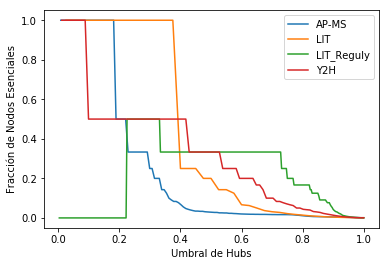
\includegraphics[width=0.5\textwidth]{figura1.png}
\label{figura1}
\caption{Fracci\'on de nodos esenciales sobre el total de hubs, en funci\'on de la fracci\'on de hubs sobre el total de nodos, para distintos umbrales de definici\'on de hubs.}
\end{figure}

Como se puede apreciar, la proporci\'on de nodos esenciales entre los hubs se incrementa a medida que el umbral de definici\'on de los hubs se hace m\'as restrictivo. Esto indica que, en proporci\'on, hay m\'as nodos esenciales cuanto mayor es el grado de los nodos considerados. Esto no se cumple estrictamente para la red LitReguly, que no contiene nodos esenciales para grado m\'aximo. Por lo dem\'as, en las dem\'as redes se observa el cumplimiento estricto de la regla de centralidad y letalidad. Zotenko complementa este an\'alisis cualitativo con la determinaci\'on de dos coeficientes de correlaci\'on, pero aqu\'i omitiremos este paso.

Dado que la regla de centralidad y letalidad se cumple en todas las redes analizadas (aunque en menor medida para la red LIT\_Reguly), es posible emplearlas para analizar con mayor detalle los modelos explicativos propuestos por Jeong y He.


\section{An\'alisis de vulnerabilidad}

Tal como se adelant\'o en la introducci\'on, la hip\'otesis de Jeong es que la esencialidad de las prote\'inas se debe a que mantienen la conectividad de la red, que a su vez est\'a asociada con el grado de los nodos.

Esta hip\'otesis tiene dos implicaciones cuya ocurrencia puede ser testeada. Si la esencialidad de las prote\'inas se debe a su rol como garantes de la conectividad global de la red, entonces, la remoci\'on de aquellos nodos que tienen una mayor centralidad medida en t\'erminos globales deber\'ia ser la forma m\'as eficaz de desarmar la componente gigante. La segunda implicaci\'on es que la remoci\'on de los nodos esenciales deber\'ia ser m\'as efectiva que la remoci\'on de los nodos no esenciales. Como veremos a continuaci\'on, ninguna de las dos cosas sucede. 


\subsection{Desarme de la componente gigante}

Una de las consecuencias de la hip\'otesis de Jeong es que las prote\'inas esenciales deber\'ian tener un alto grado de centralidad, medida a trav\'es de distintos \'indices y entonces, la remoci\'on de los nodos con mayor centralidad deber\'ia ser m\'as eficiente para el desarme de la componente gigante. En efecto, Zotenko y colaboradores mostraron que la betweenness es un mejor predictor de centralidad que el grado de los nodos. Por ende, estudiamos el desarme de la componente gigante de las cuatro redes, utilizando tres formas distintas de medir la centralidad de los nodos: grado, eigenvector y betweenness. Las primeras dos son medidas locales, asociadas con el comportamiento en el vecindario de cada nodo, mientras que la tercera es una medida global, relacionada con el rol de conectividad que los nodos desempe\~nan en la red. Ahora bien, si las prote\'inas esenciales que son los hubs realmente tienen un rol preponderante en la conectividad global de la red, esperar\'iamos que el criterio de sacar los nodos que tienen mayor betweenness fuera el m\'as eficiente para el desarme de la componente gigante.

Para testear esto lo que hicimos fue tomar cada red y desarmar la componente gigante del siguiente modo: en cada paso de iteraci\'on se removi\'o aquel modo que tuviese el mayor valor de centralidad, seg\'un cada uno de los tres \'indices medidos. Luego el proceso se repiti\'o sobre sobre la componente gigante residual una y otra vez hasta desarmarla completamente. Adem\'as de usar los tres criterios de centralidad, se implement\'o un proceso random, el cual consist\'ia en desarmar la componente gigante quitando nodos al azar. Los resultados del proceso se pueden consultar en la Fig. \ref{figura2}. Se puede advertir que todas las redes son robustas frente al desarme random. Esta propiedad ha sido atribuida en general a las distribuciones libres de escala [Jeong]. Sin embargo, se puede apreciar que el criterio m\'as efectivo para el desarme no es la betweenness, sino el grado de los nodos. Esto no est\'a de acuerdo con lo que esper\'abamos en caso de que la hip\'otesis de Jeong fuera correcta, ya que la betweenness es un. Por el contrario, esta circunstancia sugiere que no lo es y que los hubs est\'an asociados con efectos locales de su propio vecindario en lugar de estarlo con la conectividad global de la red. Este comportamiento inconsistente fue indicado no solamente por Zotenko y colaboradores, sino tambi\'en por He y colaboradores.


\begin{figure}
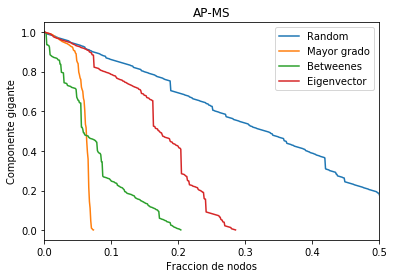
\includegraphics[width=0.45\textwidth]{figura2a.png}\\
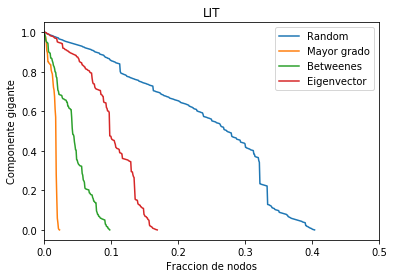
\includegraphics[width=0.45\textwidth]{figura2b.png}\\
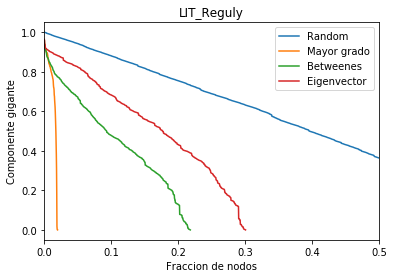
\includegraphics[width=0.45\textwidth]{figura2c.png}\\
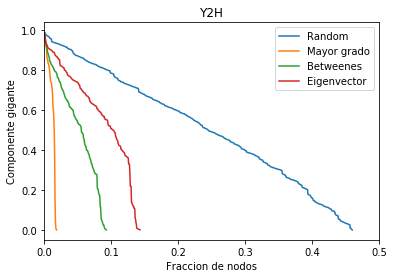
\includegraphics[width=0.45\textwidth]{figura2d.png}\\
\label{figura2}
\caption{Tama\~no de la componente gigante en funci\'on del n\'umero de nodos removidos de acuerdo con distintos criterios de centralidad de nodos en la red.}
\end{figure}

\subsection{Impacto diferenciado}

Una segunda implicancia de la hip\'otesis de Jeong es que, si los nodos esenciales son efectivamente responsables de la conectividad de la red, esperar\'iamos que el desarme de la componente gigante fuera m\'as eficiente al considerar solamente prote\'inas esenciales que al considerar un n\'umero equivalente de prote\'inas no esenciales. Es decir, esperar\'iamos que el impacto de remover hubs fuera m\'as grande para nodos esenciales que para nodos no esenciales.

Para poner a prueba esta idea lo que hicimos fue una variante de la idea de Zotenko. Para cada una de las redes consideradas, desarmamos la componente gigante de dos maneras distintas. Por un lado, la desarmamos quitando un n\'umero dado de prote\'inas esenciales al azar. Por otro, la desarmamos quitando nodos no esenciales al azar, pero respetando la misma distribuci\'on de grado que ten\'ian las prote\'inas esenciales removidas. Este proceso se repiti\'o para distinto n\'umero de nodos removidos. En la Fig. \ref{figura3} se puede ver un gr\'afico del tama\~no de la componente gigante residual en funci\'on del n\'umero de prote\'inas removidas al azar, fueran esenciales (rojo) o no esenciales (azul), para cada una de las cuatro redes. Se puede ver claramente que la remoci\'on de los nodos esenciales es tan eficiente como la remoci\'on de nodos no esenciales. M\'as a\'un, en la red LIT\_Reguly los nodos no esenciales son m\'as eficientes que los esenciales. Por consiguiente, esto suministra evidencia adicional contraria a la hip\'otesis de Jeong.


\begin{figure}
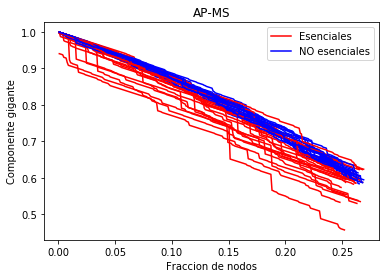
\includegraphics[width=0.45\textwidth]{figura3a.png}\\
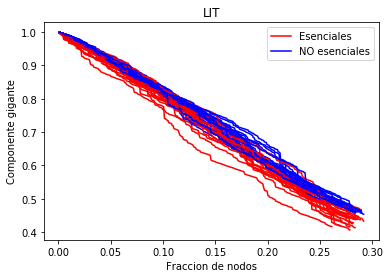
\includegraphics[width=0.45\textwidth]{figura3b.png}\\
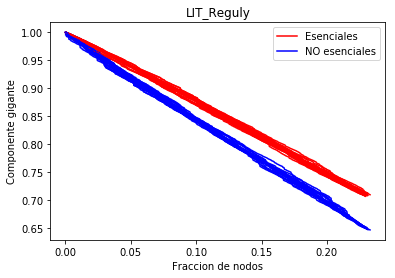
\includegraphics[width=0.45\textwidth]{figura3c.png}\\
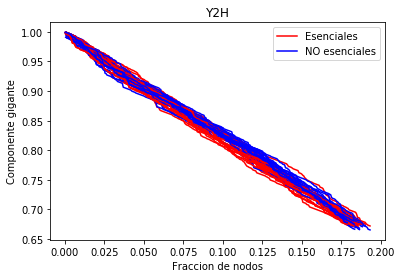
\includegraphics[width=0.45\textwidth]{figura3d.png}\\
\caption{Tamaa\~no de la componente gigante residual en funci\'on del n\'umero de nodos removidos al azar, seg\'un sean esenciales (rojo) o no esenciales (azul).}
\label{figura3}
\end{figure}

\section{Esencialidad: M\'odulos biol\'ogicos vs. Interacciones esenciales}

La hip\'otesis de He pretend\'ia explicar la regla de Centralidad-letalidad sin apelar a la arquitectura de la red proteica. Para eso, postulaba la existencia de enlaces esenciales, distribuidos aleatoriamente a trav\'es de la red de interacciones. A partir de esta idea, He y sus colaboradores desarrollaron un modelo que predice la probabilidad de que una prote\'ina al azar resulte esencial, en t\'erminos de:

\begin{enumerate}
\item La probabilidad de que los enlaces de la prote\'ina sean esenciales (lo cual depende indirectamente del grado k de la prote\'ina en cuesti\'on) y
\item La probabilidad de que la prote\'ina resulte esencial por otros motivos. 
\end{enumerate}

El modelo propuesto es

\begin{equation}
P_E = 1 -�� (1-\alpha)^k(1-\beta)
\label{eq1}
\end{equation}

He estim\'o $\alpha$ y $\beta$ utilizando dos m\'etodos alternativos, cuyos resultados demostraron ser consistentes incluso para distintas redes (es decir, los valores de cada red, determinados por distinto m\'etodo coincid\'ian razonablemente, aunque difirieran de una red a otra). En este trabajo, lo que hicimos fue utilizar uno de los m\'etodos empleados por He: graficar la fracci\'on de nodos esenciales en funci\'on del grado, linealizar la ec. \ref{eq1}, realizar un ajuste por m\'inimos cuadrados y calcular $\alpha$ y $\beta$ a partir de la pendiente y la ordenada al origen de la recta de ajuste. Los resultados del ajuste para cada una de las redes se muestran en la Fig. \ref{figura4}, mientras que los valores de $\alpha$ y $\beta$ se resumen en la tabla \ref{tabla3}. Los valores difieren de una red a otra, aunque dos de estas redes tienen valores cercanos entre s\'i. En particular, los valores m\'as peque\~nos est\'an de acuerdo con los reportados por He y colaboradores, especialmente para la red LIT\_Reguly. 

\begin{figure}
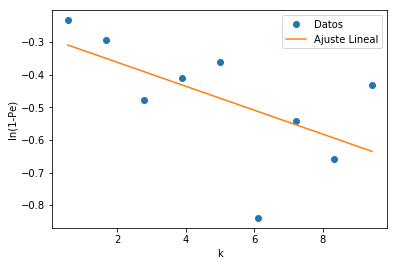
\includegraphics[width=0.45\textwidth]{figura4a.png}\\
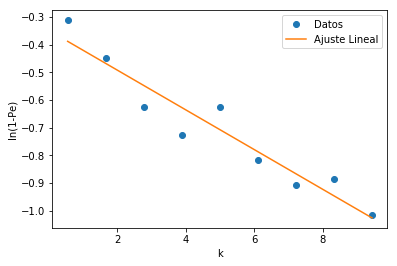
\includegraphics[width=0.45\textwidth]{figura4b.png}\\
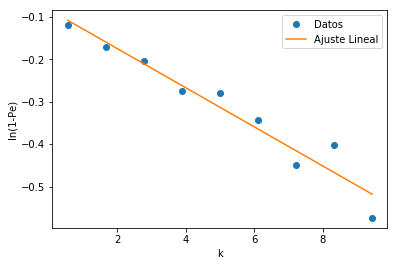
\includegraphics[width=0.45\textwidth]{figura4c.png}\\
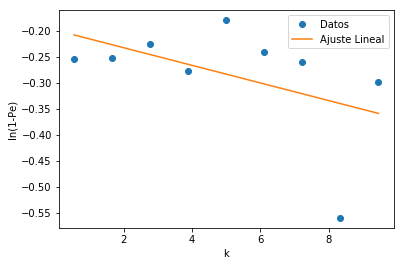
\includegraphics[width=0.45\textwidth]{figura4d.png}\\
\caption{Fracci\'on de nodos no esenciales en funci\'on del grado de cada uno de los nodos, visualizado en escala logar\'i�tmica. La recta de color naranja corresponde al ajuste por m\'i�nimos cuadrados empleando la versi\'on linealizada de la ec. \ref{eq1}.}
\label{figura4}
\end{figure}


\begin{table}[h]
\begin{ruledtabular}

\begin{tabular}{ c l c l c  }
{}&           {\bf     $\alpha$ }&{\bf     $\beta$}\\\hline\\
{\bf AP-MS   }&{    0.25}&{  0.036}\\
{\bf LIT   }&{     0.29  }&{0.069}\\
{\bf LIT\_Reguly }&{ 0.079 }&{ 0.045}\\
{\bf Y2H      }&{   0.18 }&{ 0.017}\\
\end{tabular}
\end{ruledtabular}
\caption{Valores de los coeficientes $\alpha$ y $\beta$ obtenidos del ajuste por cuadrados m\'i�nimos, para cada una de las cuatro redes.}
\label{tabla3}
\end{table}

Sin embargo, Zotenko se\~nal\'o que el modelo de He parte de una hip\'otesis central: se asume que la probabilidad de que una dada prote\'ina sea esencial es independiente de la probabilidad que tiene, de ser esencial, cualquier otra prote\'ina no enlazada con ella. Si esto fuera cierto, entonces esperar\'iamos que no haya correlaciones entre la cantidad de pares de prote\'inas esenciales y la cantidad de pares de prote\'inas no esenciales. Es decir, la cantidad de pares predichas por el modelo de He deber\'ia ser similar a la cantidad de pares efectivamente encontrados en la red.

Para testear esta idea tomamos las redes originales y calculamos la cantidad de pares de prote\'inas no enlazadas, tales que tuvieran al menos tres vecinos comunes y que compartieran el mismo grado de esencialidad (ambas esenciales o ambas no esenciales). Luego, se utilizaron los $\alpha$ y$\beta$estimados en el punto anterior para determinar qu\'e cantidad de prote\'inas con igual grado de esencialidad cabr\'ia esperar si el modelo de He fuese correcto. La cantidad de estos pares se determin\'o simplemente como el producto entre la cantidad total de pares de prote\'inas en la red por la probabilidad de que dos prote\'inas tengan el mismo grado de esencialidad. Esto es:

\begin{equation}
N_{est} = N_T [P_E^2+(1-P_E)^2]
\end{equation}

Los resultados comparados se pueden encontrar en la tabla \ref{tabla4}. Se puede observar que la cantidad de pares de prote\'inas con el mismo grado de esencialidad que efectivamente se encontr\'o en la red es significativamente menor que la cantidad de pares predichos por el modelo de He para las redes AP-MS y LIT, mientras que la relaci\'on se invert\'ia para las redes Y2H y LIT\_Reguly. Estos resultados contradicen lo encontrado por Zotenko, si bien Zotenko no analiz\'o exactamente el mismo tipo de redes y los resultados coinciden en la red Y2H, que s\'i tenemos en com\'un con dicho trabajo. Como consecuencia de lo antedicho, no es posible refutar el modelo de He, ni tampoco corroborarlo, ya que la evidencia no es conclusiva al respecto. 

\begin{table}[h]
\begin{ruledtabular}
\begin{tabular}{ c l c l c l c }  
{}&{\bf          \# total }&{\bf  \# de pares }&{\bf \# Esperado }\\
{}&{\bf          de pares}&{\bf  del mismo tipo }&{\bf  (ajuste lineal)  }\\\hline\\
{\bf AP-MS        }&{           12646           }&{             6957 }&{  11951 }\\
{\bf LIT            }&{          1392          }&{              1055  }&{ 1099}\\
{\bf LIT\_Reguly      }&{        12251             }&{ 7660   }&{ 7414}  \\
{\bf Y2H}&{978 }&{808}&{632}\\

\end{tabular}
\end{ruledtabular}
\caption{Cantidad de pares con igual grado de esencialidad (ambas esenciales o ambas no esenciales) tanto para las redes reales como predichas por el modelo de He y colaboradores.}
\label{tabla4}
\end{table}

\section{Conclusiones}

Se estudiaron cuatro redes de prote\'inas de la levadura {\sc}, a efectos de revisar cr\'iticamente dos propuestas de explicaci\'on para la regla de centralidad y letalidad. En el caso del modelo propuesto por Jeong y colaboradores, se determin\'o que no hay una relaci\'on directa entre esencialidad y conectividad, puesto que medidas m\'as sofisticadas de conectividad como la betweenness no son tan buenos predictores de esencialidad como el grado de los nodos. De hecho, los nodos esenciales y no esenciales no difieren en cuanto a su eficiencia en el desarme de la componente gigante. Esto sugiere que la esencialidad est\'a asociada con un efecto local del nodo sobre sus vecinos. 

En cuanto al modelo de He y colaboradores, se determin\'o que part\'ia de la hip\'otesis de que la probabilidad de que una prote\'ina fuera esencial era independiente de la probabilidad que tuvieran cualesquiera prote\'inas no enlazadas con ella. Al testear esta hip\'otesis se determin\'o que la cantidad de pares de prote\'inas no enlazadas con igual grado de esencialidad en la red real era significativamente inferior a la que predec\'ia el modelo de He para la mitad de las redes, pero la relaci\'on se inver\'ia para la otra mitad. En consecuencia, la hip\'otesis no pudo refutarse ni aceptarse por falta de evidencia concluyente al respecto.



\begin{thebibliography}{10}

\bibitem{Jeong}
Jeong H., Mason S. P., Barabási, A. L., Oltvai Z. N. {\em Lethality and centrality in protein networks}. Nature Brief Communications, 2001 May; 411:41-42.

\bibitem{He}
He X., Zhang J.
\newblock {\em Why Do Hubs Tend To Be Essential in Protein Networks?} PLoS Genetics. 2006 Jun; 2(6):e88.

\bibitem{Zotenko}
Zotenko E., Mestre J., O'Leary D. P., Przytycka T. M.
\newblock {\em Why do Hubs in the Yeast Protein Interaction Network Tend To Be Essential: Reexamining the Connection between the Network Topology and Essentiality}.
\newblock PLoS Computational Biology. 2008 Aug; 4(8):e1000140.

\end{thebibliography}

\end{document}
%
% ****** End of file apssamp.tex ******
